\section{Detalhamento do \textit{Design}}
\label{sec:detalhamento-design}

No \textit{design} do BROV foram levados em consideração o baixo custo e a versatilidade para futuras integrações de novos sensores. Dessa forma, optou-se por utilizar estrutura tubular de PVC, da linha de soldável da Tigre \cite{Tigre2009}. As dimensões máximas do BROV foram fixadas em 254 x 465 x 650 mm, como mostra a Figura \ref{fig:brov-dimensions}. O volume externo foi calculado em 76,7 l e a massa fora d'água em 9,2 kg.

\begin{figure}[h]
	\centering
	\caption[Vistas e dimensões máximas do BROV]{Vistas e dimensões máximas do BROV}
	\label{fig:brov-dimensions}
	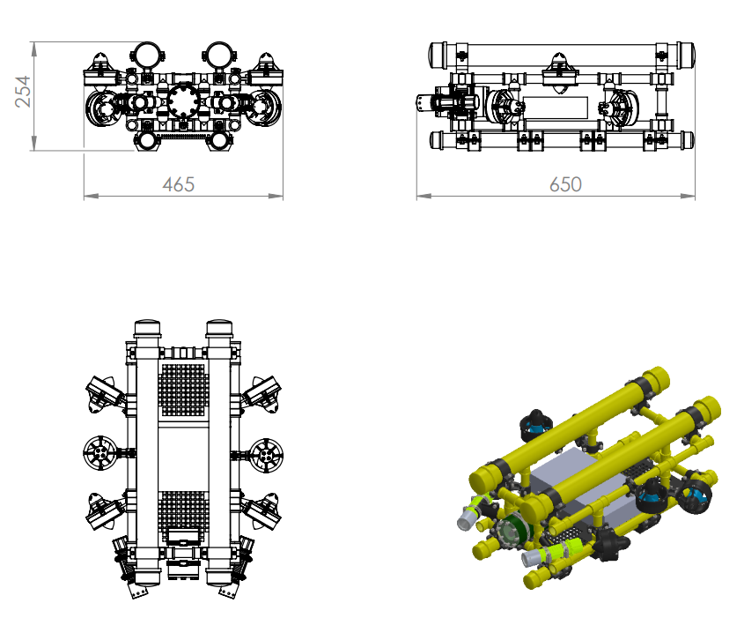
\includegraphics[width=1\linewidth]{images/brov-dimensions}\\
	\footnotesize Fonte: Autores
\end{figure}

A altura do centro de gravidade (CG) do protótipo foi calculada em 149,7 mm em relação à base, o que equivale a 59\% da altura total. Essa altura, no entanto, pode ser ajustada com adição de massa discreta nos tubos inferiores, e/ou com adição de espuma de poliuretano nos tubos superiores. A Figura \ref{fig:brov-cg-lateral} mostra uma vista lateral do BROV com indicação do CG.

\begin{figure}[h]
	\centering
	\caption[CG representado em vista lateral]{CG representado em vista lateral}
	\label{fig:brov-cg-lateral}
	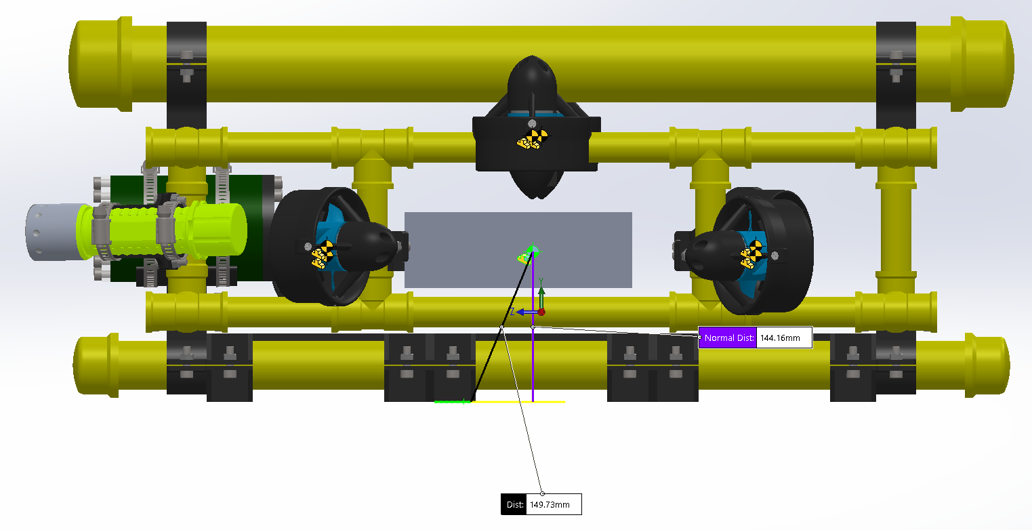
\includegraphics[width=1\linewidth]{images/brov-cg-lateral}\\
	\footnotesize Fonte: Autores
\end{figure}

Levando-se em consideração versatilidade e facilidade de montagem, o BROV foi modularizado em cinco submontagens:
\vspace{1ex}
\begin{enumerate}
	\item Estrutura;
	\item \textit{Thrusters};
	\item \textit{Housing} principal;
	\item \textit{Housing} da câmera;
	\item Lanternas.
\end{enumerate}
\vspace{1ex}

A estrutura compreende os tubos, os conectores e a base impressos 3D, e os elementos de fixação -- parafusos e porcas. Os \textit{thrusters} são compostos pelo motor \textit{brushless} A2212/13V 1000KV, hélice, peças impressas e elementos de fixação. A \textit{housing} principal acomoda toda a eletrônica do protótipo e a \textit{housing} da câmera acomoda a câmera e seu controlador. Já as lanternas são montadas a parte, fixadas por abraçadeira metálica e com fonte de alimentação independente. A Figura \ref{fig:brov-submontagens} mostra as submontagens que compõem o BROV.

\begin{figure}[h]
	\centering
	\caption[Submontagens que compõem o BROV]{Submontagens que compõem o BROV}
	\label{fig:brov-submontagens}
	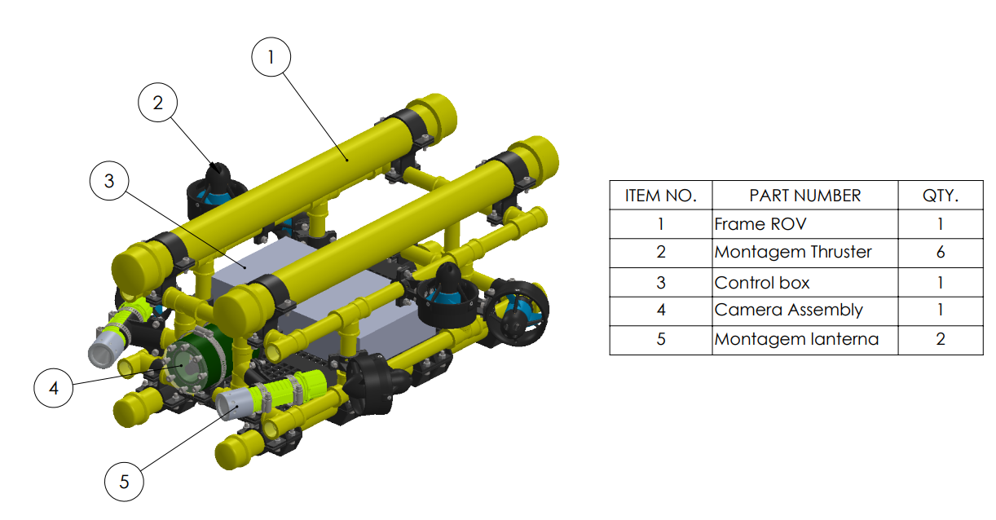
\includegraphics[width=1\linewidth]{images/brov-submontagens}\\
	\footnotesize Fonte: Autores
\end{figure}

O principal valor que a equipe agregou em termos de \textit{design} foi no \textit{thruster}. A partir do \textit{design} do \textit{thruster} T200, da \textit{BlueRobotics} (\textit{open source}), a equipe remodelou alguns componentes e fixadores, de modo a tornar possível a alocação do motor \textit{brushless} A2212/13V 1000KV. Enquanto o T200 custa atualmente cerca de R\$ 900,00 sem frete, o \textit{thruster} desenvolvido pela equipe possui um custo estimado R\$ 90,00. A Figura \ref{fig:thruster-brov-bluerobotics} mostra a comparação dos dois \textit{thrusters} e a Figura \ref{fig:brov-thruster} mostra o \textit{thruster} do BROV nas vistas isométrica e de corte.

\begin{figure}[h]
	\centering
	\caption[\textit{Thruster} T200 BlueRobotics x \textit{Thruster} BROV]{\textit{Thruster} T200 BlueRobotics x \textit{Thruster} BROV}
	\label{fig:thruster-brov-bluerobotics}
	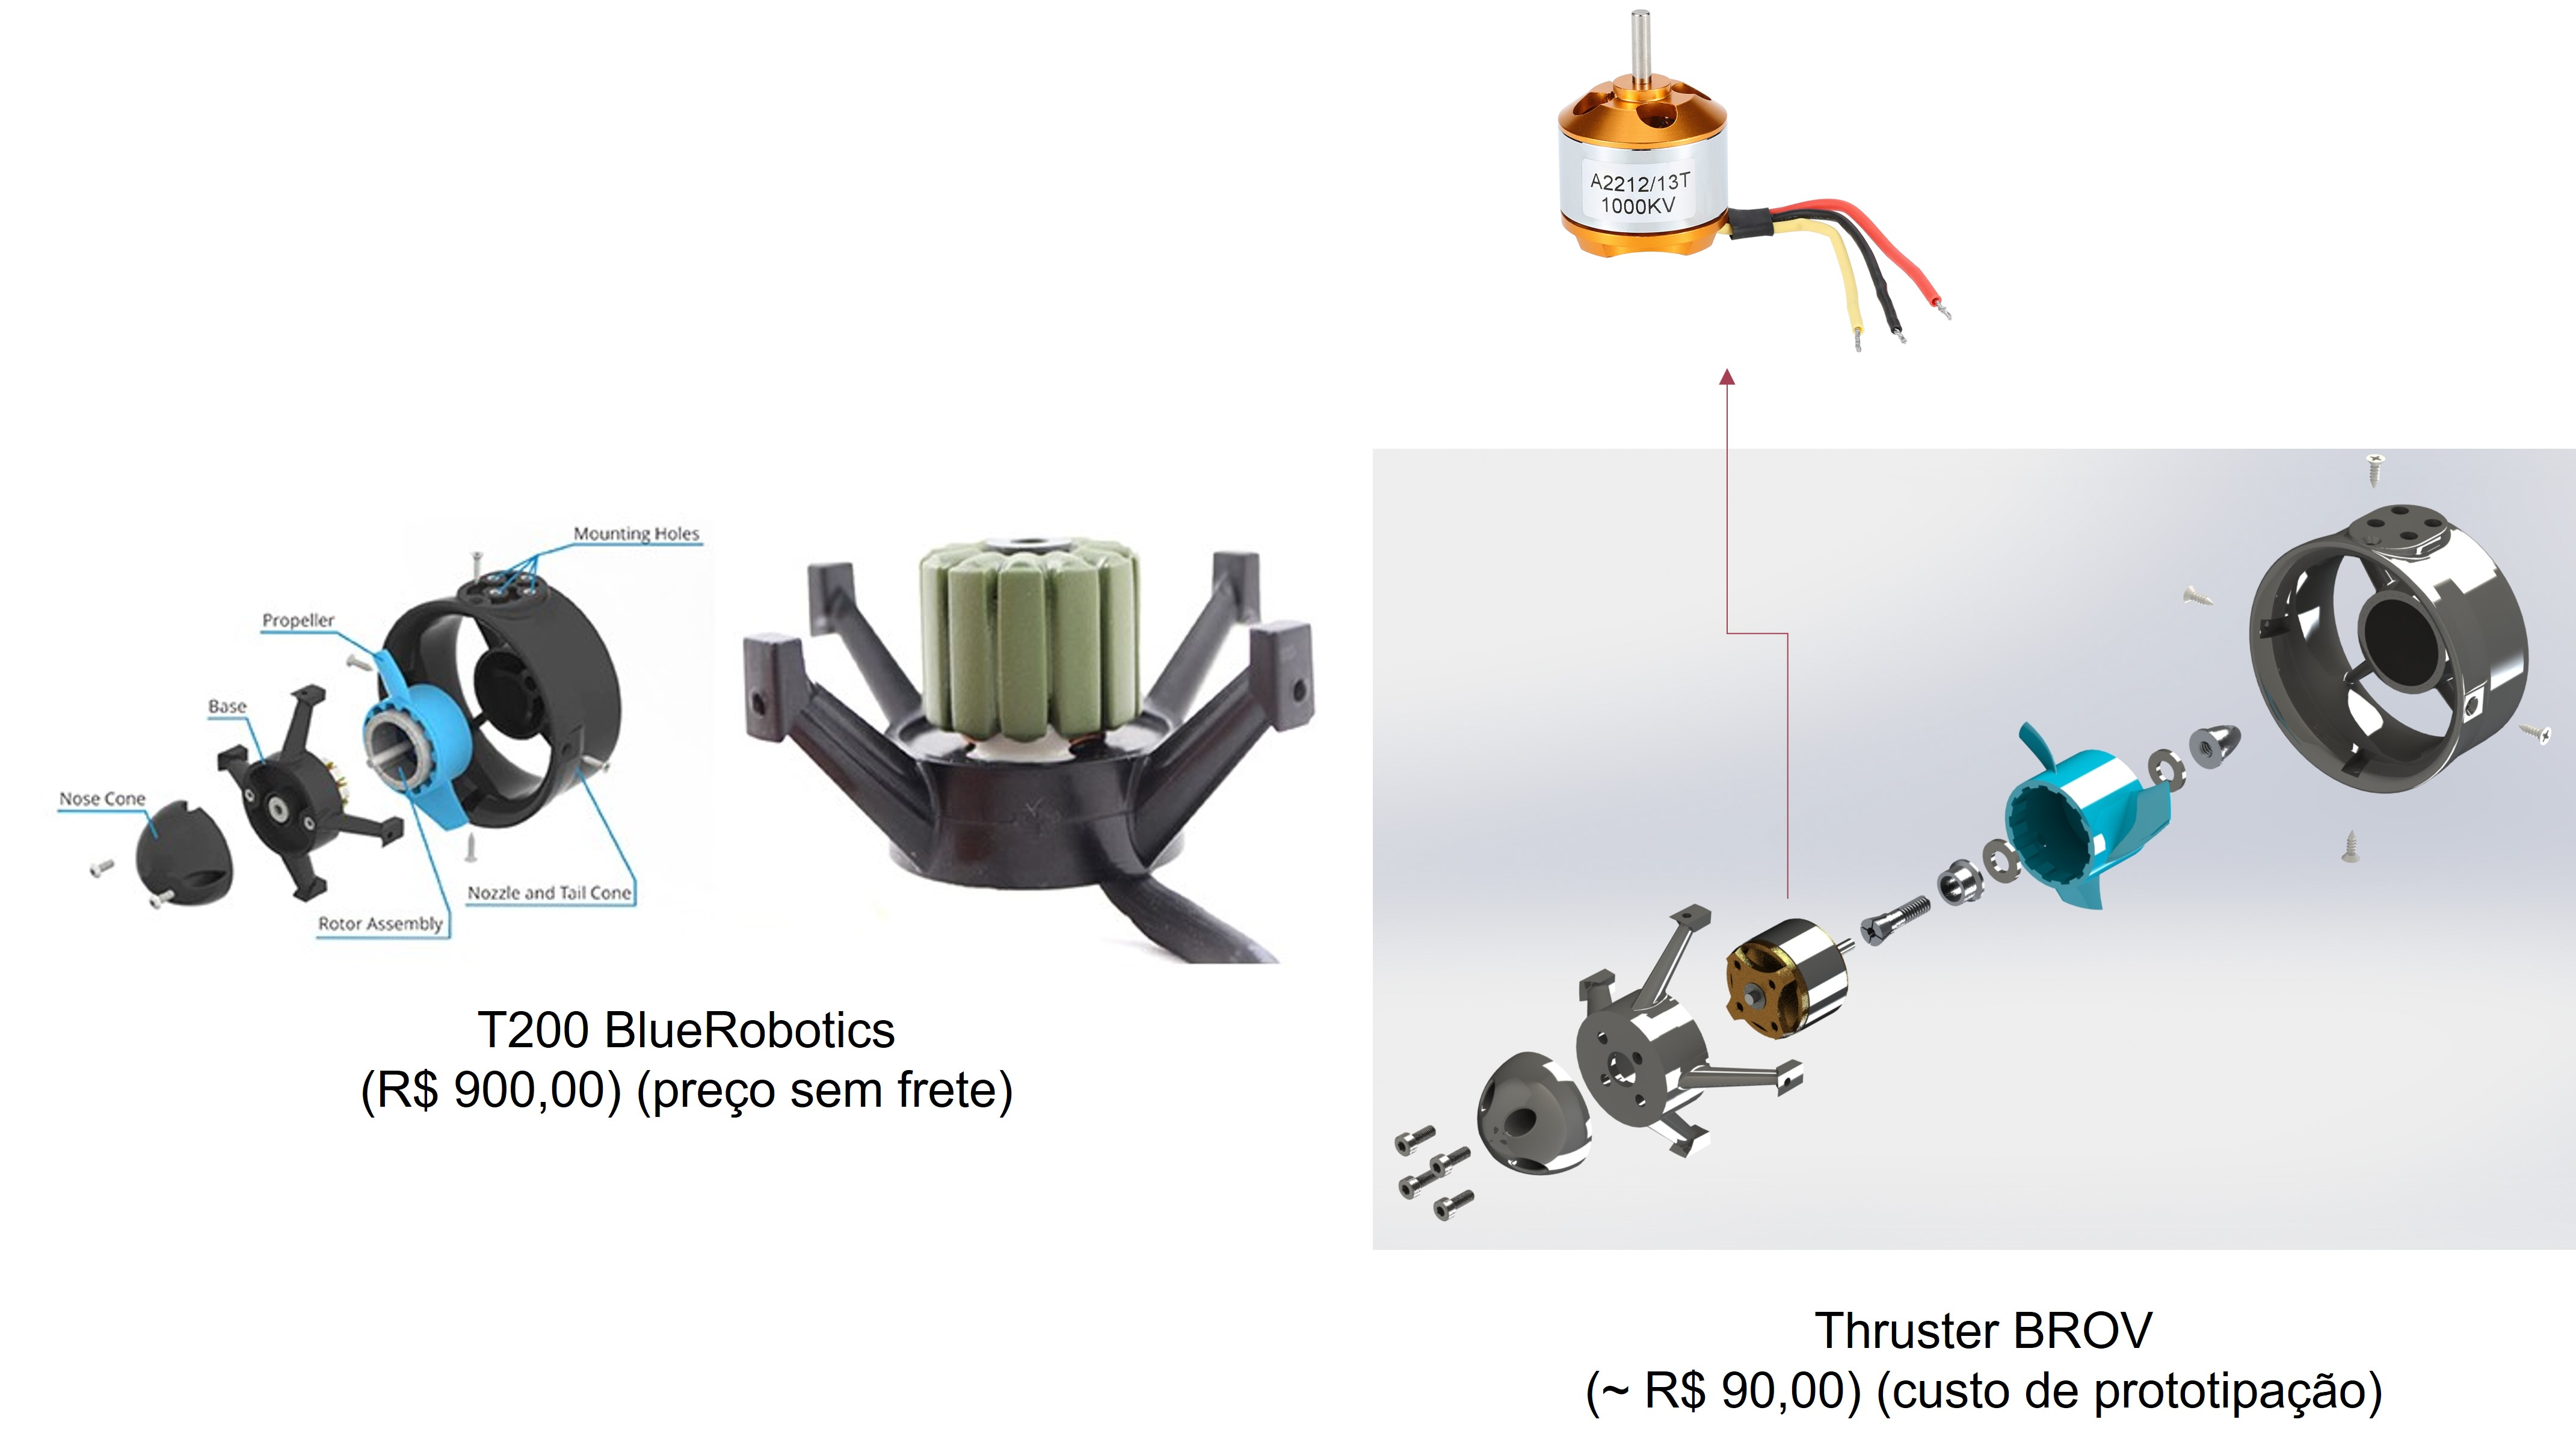
\includegraphics[width=1\linewidth]{images/thruster-brov-bluerobotics}\\
	\footnotesize Fonte: Autores
\end{figure}

\begin{figure}[h]
	\centering
	\caption[Vistas isométrica e de corte do \textit{thruster} do BROV]{Vistas isométrica e de corte do \textit{thruster} do BROV}
	\label{fig:brov-thruster}
	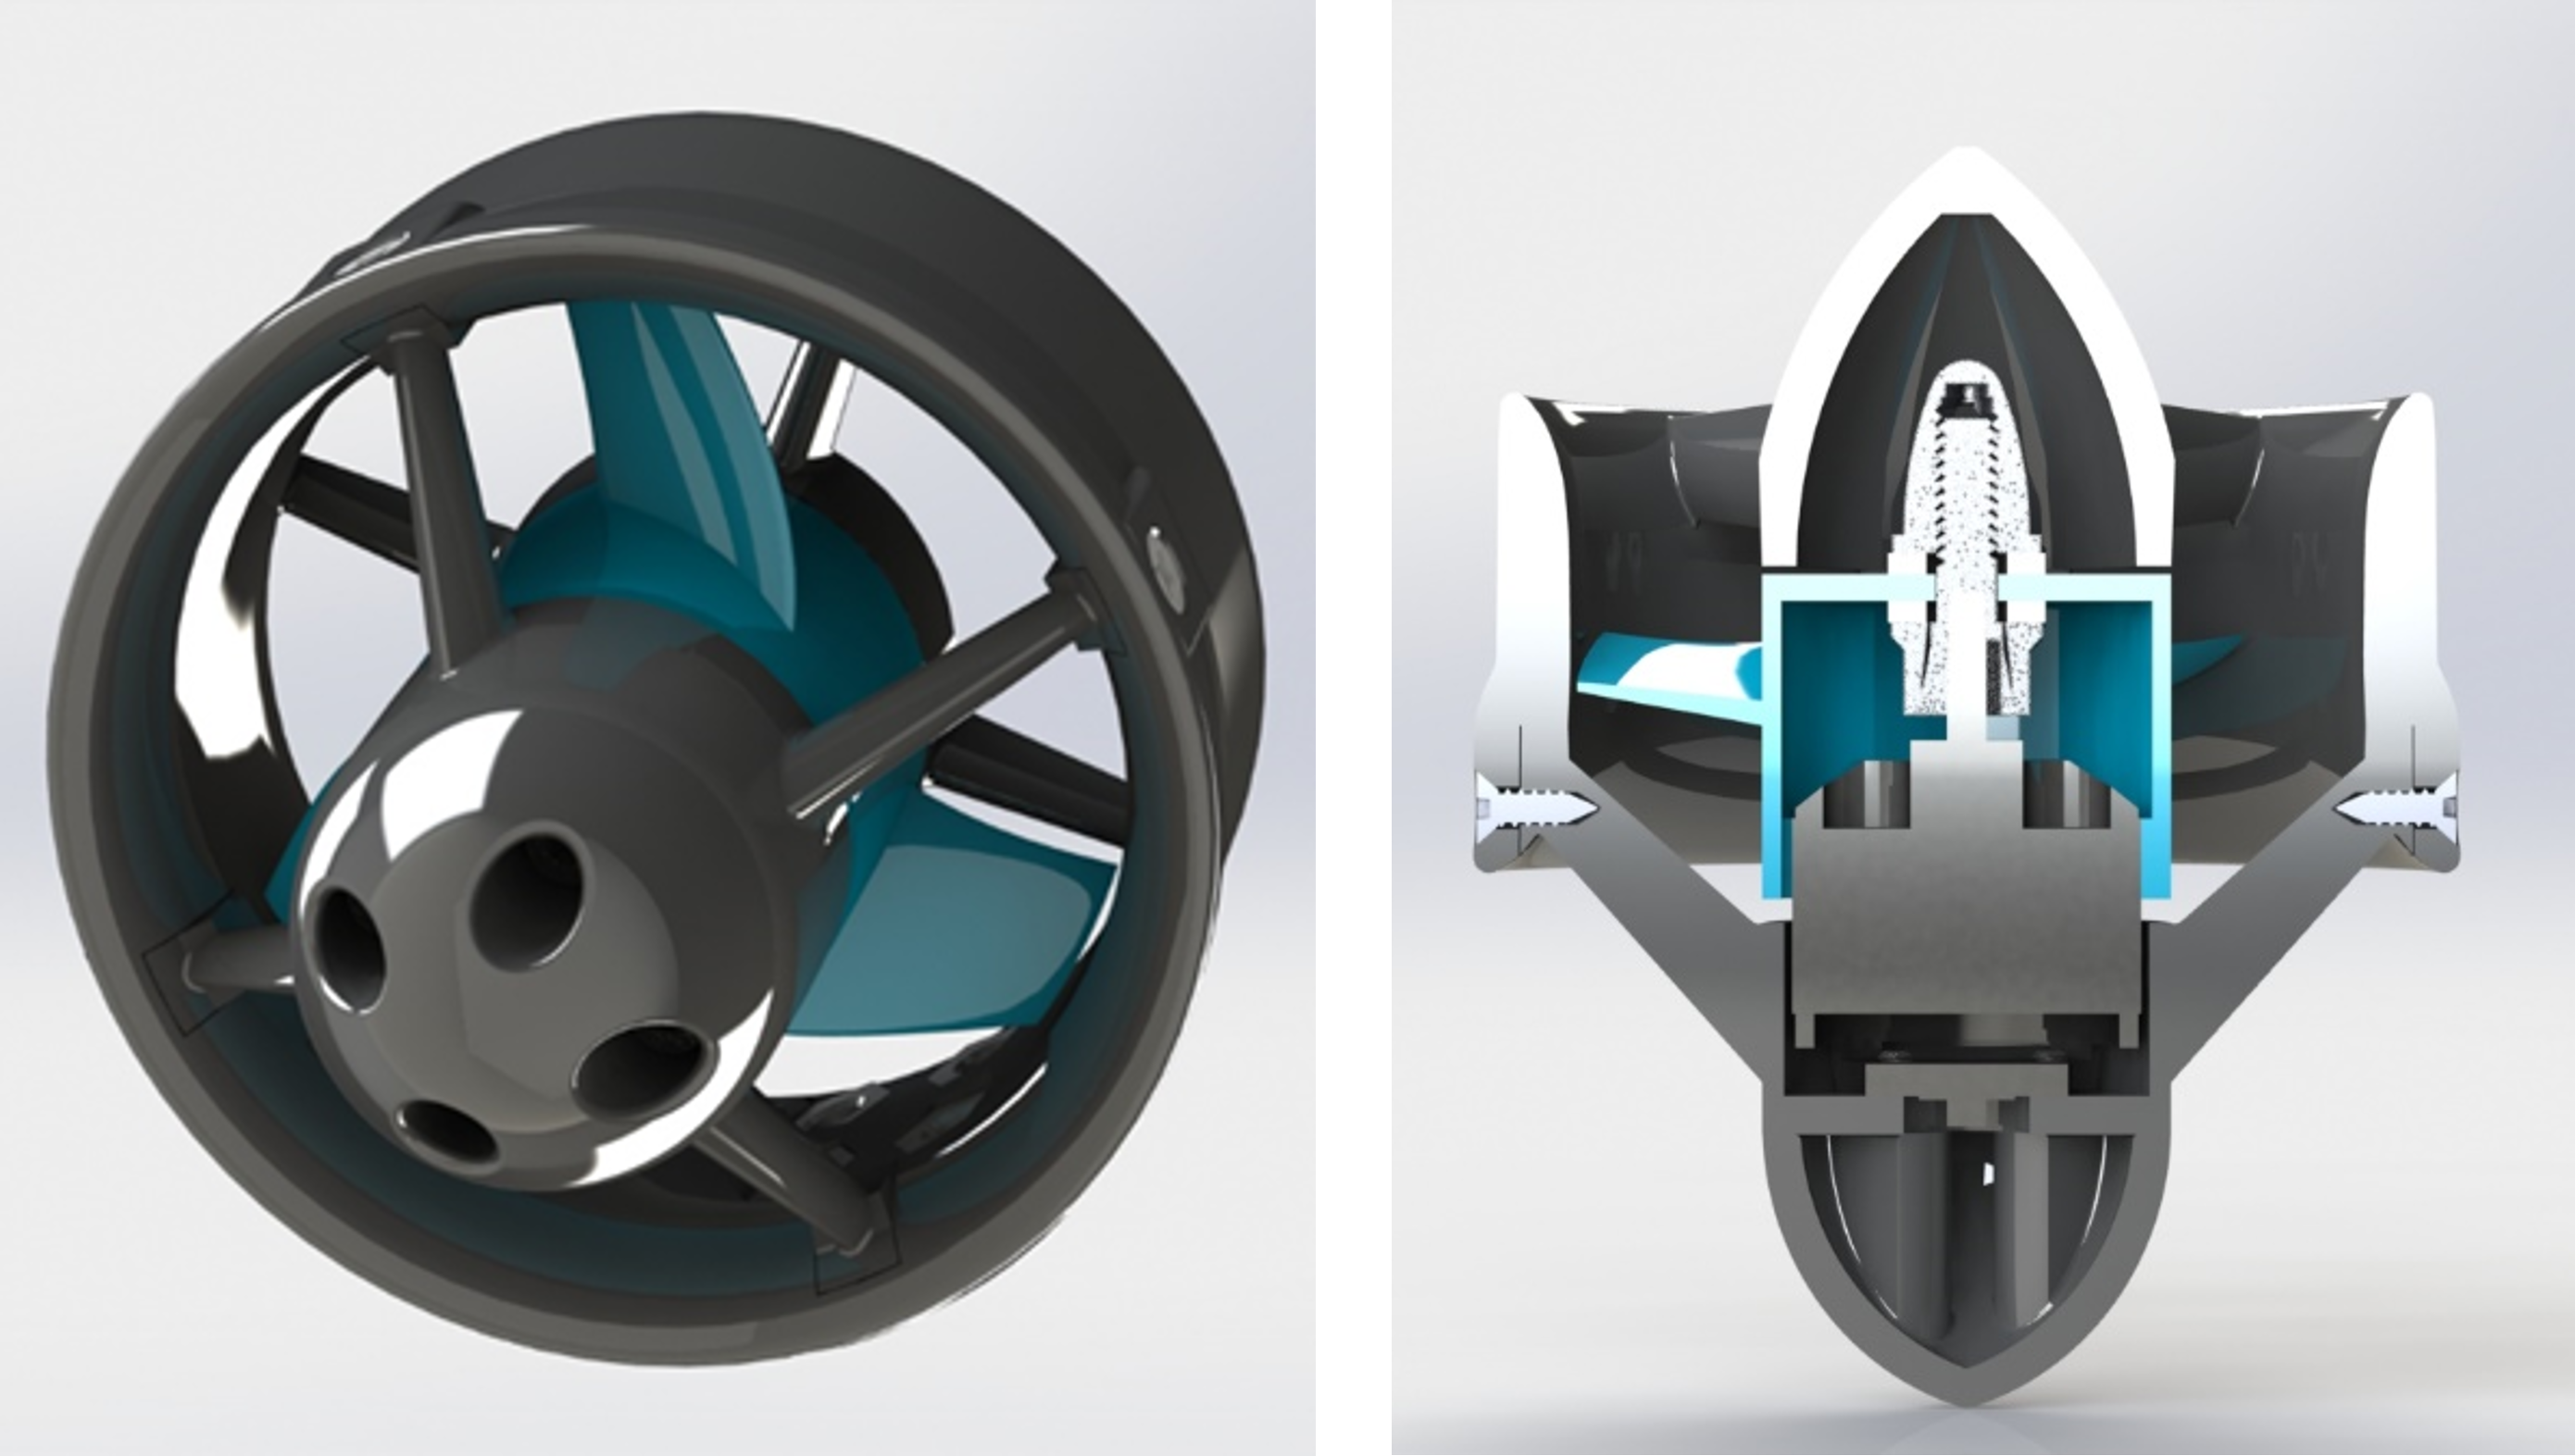
\includegraphics[width=0.8\linewidth]{images/brov-thruster}\\
	\footnotesize Fonte: Autores
\end{figure}

A Figura \ref{fig:brov-exploded} mostra a vista explodida do BROV, com a maioria dos seus componentes já modelados.

\begin{figure}[h]
	\centering
	\caption[Vista explodida do BROV]{Vista explodida do BROV}
	\label{fig:brov-exploded}
	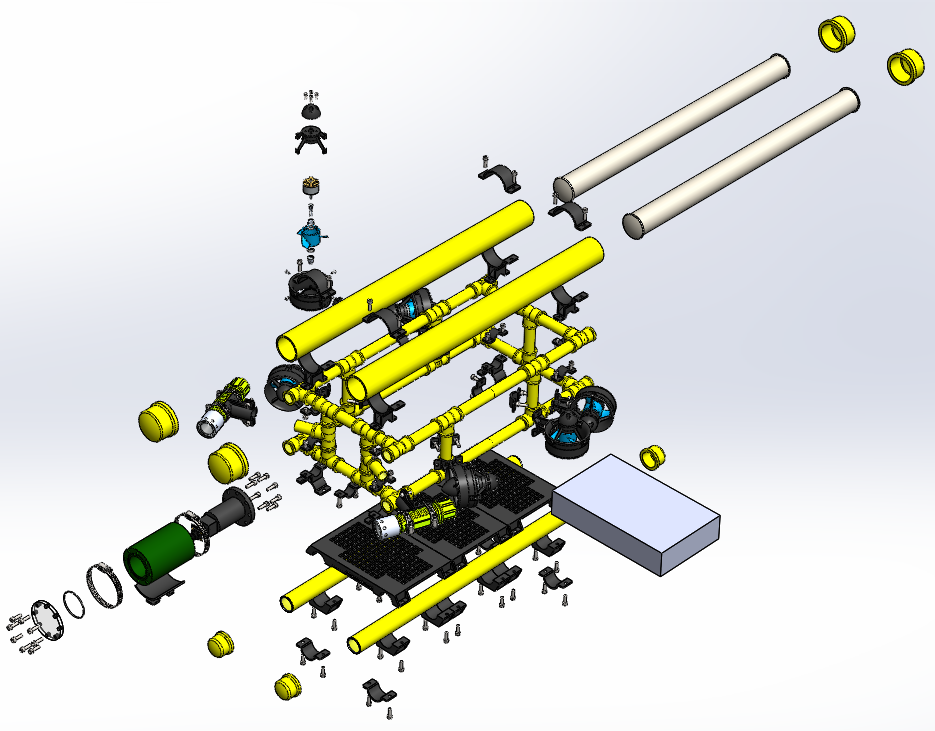
\includegraphics[width=1\linewidth]{images/brov-exploded}\\
	\footnotesize Fonte: Autores
\end{figure}

